\chapter{Background and selection criteria}
\label{chp:LitSurvey}
In this chapter, a state-of-the art study will be presented that could assist in design of the lensless imager with specifications mentioned in the previous chapter.
\section{Camera Computational Pipeline}
In order to design a lensless imaging system, we must first look at the computational imaging pipeline of existing cameras. Since the lensless camera basically uses computation to reconstruct images, it is important to understand the computational pipeline of existing camera systems and make necessary modification in the design of the existing pipeline to suit the system. The computational imaging pipeline of existing camera systems is shown figure \ref{fig:CompPipeline}\cite{CompPipeline}.
\begin{figure}[htb]
% most GNUplot figures need to be rotated, width should be the same throughout the complete document, and no extension is needed
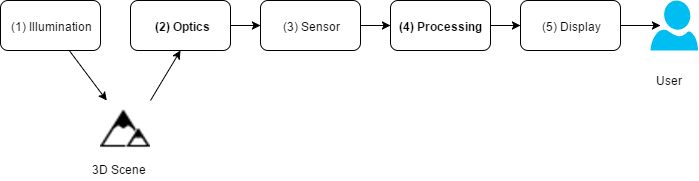
\includegraphics[width=\textwidth]{pics/CompPipeline}
\caption{Computational Pipeline of Existing cameras}
\label{fig:CompPipeline}
\end{figure}
As shown in figure \ref{fig:CompPipeline}, there are five main components that can be controlled computationally in existing systems. Illumination of the scene can be controlled to produce an enhanced picture. Optics could be controlled to limit the amount of light entering the scene and thereby controlling the image produced on the sensor. The sensor can also computationally modify the date it receives to de-noise, adjust the blackness/white in an image. Post-processing can also be done on the image produced by the sensor to improve the image produced by the sensor. Finally, a display can also be modified computationally to produce certain effects on the user. And of course, the user can control any of these components to produce the effect he desires. But in the case of the lensless imaging system, we would be modifying the optics and the processing components of the pipeline to reduce the size of the camera.The components to be modified are are darkened in figure \ref{fig:CompPipeline}. 

\section{Satellite Imaging Architectures}
Since the camera is going to be capturing pictures of the earth, it would be required to study the existing imaging architectures currently being used in satellites and how the design of the lensless camera would fit into the existing imaging architectures. We will first look into the terminology commonly used in space instrumentation. As the imager is carried along the orbit of the earth, it images a strip on the surface of the earth. The width of the strip is called the 'swath'. The direction along which the satellite moves or images is called the 'along-track' direction and the direction perpendicular to it is called the cross-track direction\cite{ImagingGeo}. Figure \ref{fig:ImagingGeo} describes these terminology and some other terms as well.  
\begin{figure}[ht]
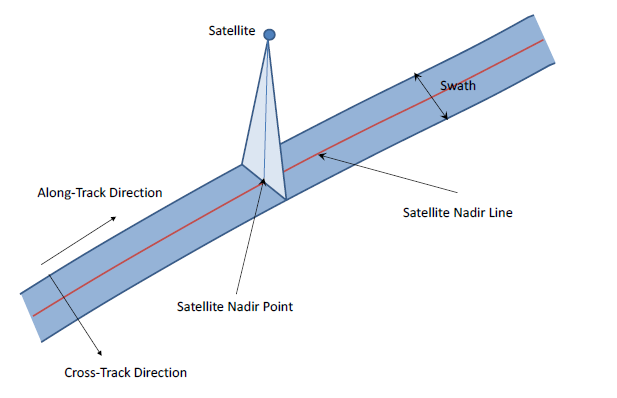
\includegraphics[width=\textwidth]{pics/imaginggeo}
\caption{Various Imaging Terms\cite{ImagingGeo}}
\label{fig:ImagingGeo}
\end{figure}
Three major types of scanning architectures are employed in space instruments, namely:
\begin{itemize}
\item Whiskbroom Line Scanner: In this type of scanning architecture, a detector element detects it's instantaneous field of view which is projected onto a pixel element. In this scanning type the surface of the earth is scanned in lines. A scanning mirror would project a very small area of the earth onto the single pixel element. The scanning mirror would then rotate to project the next element of the line onto the next pixel. Depending on the motion of the satellite, the next line of the detector is scanned and projected on to the next line on the surface of the earth. An advantage of this type of detector is that it would be possible to obtain a very large field of view. However, it also comes with disadvantage that a very high sampling frequency is required to get decent resolutions. Typically, an earth observation satellite would move at 6.5 km per second. In order to get a resolution of 100 meters per pixel, it would be required to sample atleast 65 lines per second. For a swath of 1000 pixels it would be required to sample at 65000 elements per second. Apart from this, there is very limited time for each detector element which would result in low spatial resolution\cite{SpInst}. Another main disadvantage is that mechanical components would be required to project different parts of the surface of the earth on to the detector element. This type of scanner is also called as along-track scanner. Mathematically, the measurement of the detector element $(X,Y)$ can be described using 
$$
(X,Y) = f(t_x, t_y)
$$
where $t_x$ and $t_y$ is the time at which the image is captured in the corresponding location
%\begin{figure}[ht]
%\begin{subfigure}
%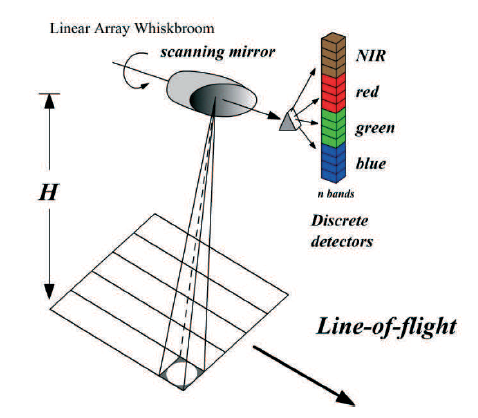
\includegraphics[width=0.5\textwidth]{pics/WhiskBroom}
%\caption{Whiskbroom Scaning Architecture}
%\label{fig:WhiskBroom}
%\end{subfigure}
%\begin{subfigure}
%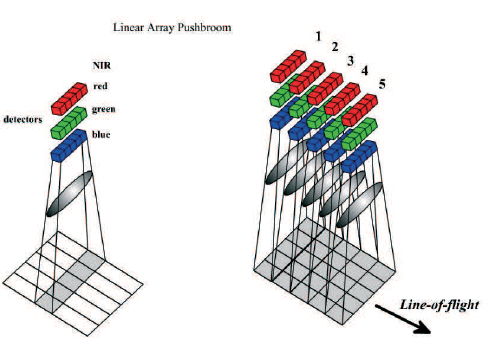
\includegraphics[width=0.5\textwidth]{pics/PushBroom}
%\caption{Pushbroom Scaning Architecture}
%\label{fig:PushBroom}
%\end{subfigure}
%\end{figure}
\begin{figure}[ht]
\centering
\begin{subfigure}{0.75\textwidth}
  \centering
  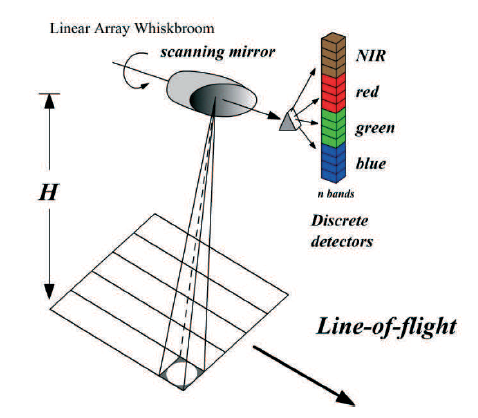
\includegraphics[width=.5\linewidth]{pics/WhiskBroom}
  \caption{WhiskBroom Scanning}
  \label{fig:Whiskbroom}
\end{subfigure}
\begin{subfigure}{0.75\textwidth}
  \centering
  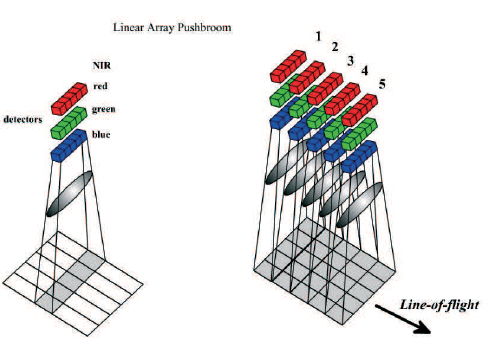
\includegraphics[width=.65\linewidth]{pics/PushBroom}
  \caption{Pushbroom Scanning}
  \label{fig:Pushbroom}
\end{subfigure}
\caption{Push Broom and Whisk Broom Scanning}
\label{fig:test}
\end{figure}

\item Pushbroom Line Scanner : In this type of architecture, the orbital motion of the sensor is used to image the swath instead of using a mirror as in the case of whiskbroom scanner. The field of view in the cross-track direction is imaged by the corresponding line detector array. Successive lines are imaged and sampled by the multiplexer as the sensor moves across the surface. The time between sampling two successive lines can be the time it takes for the satellite to move that distance. The most commonly used detector for a pushbroom scanner is Charge Coupled Devices(CCD). One of the main advantages of this type of scanner is that it requires no moving parts. Due to this, it is possible to obtain very high scanning rates(< $1 \mu$ second). This also leads to lower noise in the received signal\cite{SpInst}. The disadvantage is that large number of detectors are required to image a large piece of area. In addition to this, it requires an optical arrangement that could obtain a wide field of view. Mathematically, the measurement of the detector element $(X,Y)$ can be described using 
$$
(X,Y) = f(x), f(t_y)
$$
where $f(x)$ represents the sensor output and $f(t_y)$ represents the time at which the subsequent rows are imaged.  
\item Staring Array : Staring arrays use 2-d CCD/CMOS detectors to capture an entire area on the surface of the earth. These are also called as framing cameras. This provides speed-up and step-and-stare mechanism is employed wherein observations are made intermittently after a certain number of steps in the cross-track direction. The advantage is that moderate field of view optics is only required in this case\cite{SpInst}. Mathematically, the measurement of the detector element $(X,Y)$ can be described using 
$$
(X,Y) = f(x), f(y)
$$
where $f(x)$ and $f(y)$ represents the sensor output.
\end{itemize}
\section{Trade-off Analysis}
\label{sec:tradeOff}
\subsection{Camera Sensor}
The camera sensor is the core of the Delfi-PQ Imager. The performance of a camera is mainly limited by the image sensor that it uses\cite{cmos}. The camera sensor can be off two types namely, CCD(charge coupled device) or CMOS(Complimentary Metal Oxide Semiconductor). Both the types of CMOS sensors have their own advantages and disadvantages. To understand the challenges that each type of sensor poses, we must understand how the sensors are designed.

The following factors have been chosen to  make a trade-off between the different CMOS sensors:
\begin{enumerate}
\item Resolution : When rating a camera, the first thing that comes to the mind is the resolution of the camera. The resolution of a camera is directly dependent on the number of pixels in the image sensor of the camera. 
\item Power Consumption : In the design of the PQ-Camera, the most important factor is the power consumption of the entire imager. The majority of the power consumption by the imager is dependent on the power consumption of the CMOS sensor. 
\item Availability : Even though there are innumerable number of CMOS sensors in the world, availability of CMOS sensors is quite low when it comes to small-scale. Many CMOS manufacturers require large scale orders.
\item Quantum Efficiency(QE) : Quantum Efficiency is the measure of efficiency of the camera sensor to convert incoming photons into electrons. The ratio of electrons generated during the digitization process to photons is called quantum efficiency.
\item Pixel Size : Pixel size is the size of each pixel unit in the CMOS camera. It is also an important factor considering that the signal produced by the CMOS sensor depends on the pixel size as well.
$$
Signal = Light Density * (Pixel Size)^2 * QE
$$
\item Electronic Interface : The electronic interface that can be used to retreive data from the CMOS sensor also plays an important role. Since the project uses a low-power microcontroller that has limited communication capabilities, it would be wise to chose an interface that is supported by the microcontroller. Recently available chips use LVDS/MIPI interface to send data. These interfaces are not supported by the microcontroller that is being used as an on-board computer. The on-board computer uses an I2C based interface and that the electronic interface would be an important factor as it would reduce the complexity of the system and also reduce the power consumption by removing the addidional circuitry necessary for interfacing with the onboard computer.

\item Dynamic Range : Dynamic Range and SNR are used interchangeably in CMOS sensors. The only difference is that dynamic range considers only the temporal dark noise while SNR includes the root mean square of the shot noise as well.  

\item Shutter Type : Camera sensors use different types of shutters namely, global shutter and rolling shutter. Global shutter reduces the distortions due to fast moving artefacts while increasing the dark current. Rolling shutter has more distortions in the case of imaging moving artefacts, but also has lesser dark noise compared to global shutter. 

\item Voltage Level : Voltage level also has to be taken into account while choosing the sensor because if the CMOS sensor needs a voltage level higher than that of the main satellite bus voltage, then additional circuitry has to be introduced to step up the voltage level which in turn increases the overall system power.  

\item Operating Temperature : Operating temperature is an important factor to take into account when choosing an imaging sensor. Since the camera is going to operate in space, it is better if the CMOS sensor has a higher operating range of temperature. 

\item Overall Size and Weight : As the imager has to fit within specific dimensions, the overall size and weight of the CMOS sensor also needs to be taken into account.

\item Frame Rate: Even though, it is not required to have a camera sensor that is capable of high frame rates, it is an added advantage and higher frame rate camera could help in imaging larger areas of the earth if required. 
\item Price: While there are no specific cost constraints in the project, price has also been taken into account.
\end{enumerate}

In \cite{surveyCamMod}, a survey of camera modules for a CubeSat space Mission has already been carried. However, we also consider image sensors(not same as camera modules) as we are fundamentally changing the design of a camera. 

The following candidates have been chosen for analysis. These candidates are chosen based on \cite{surveyCamMod} and also on the latest CMOS sensors available on the market. 
\begin{enumerate}[label=(\alph*)]
\item IDS UI- 1646LE USB 1.3MP
\item C3188A
\item PC67XC-2 CCD
\item MicroCam TTL
\item PB-MV40
\item Omnivision OV7670
\item Sony ICX285AL
\item Omnivision OV5642
\item Omnivision OV2740
\item MCM20027
\end{enumerate}

\begin{table}[ht]
\caption{Comparison of Different Image Sensor Candidates}
\label{tbl:TradeoffCMOS}
\begin{tabular}{|c|c|c|c|c|c|c|c|c|c|c|}
\hline
\diaghead{\theadfont Diag ColumnmnHead II}%
{Factors}{Candidates}&
\thead{(a)}&\thead{(b)}&\thead{(c)}&\thead{(d)}&\thead{(e)}&\thead{(f)}&\thead{(g)}&\thead{(h)}&\thead{(i)}&\thead{(j)}\\
\hline
\textbf{Optical Parameters} & & & & & & & & & &\\
\hline
Resolution & ++ & + & + & - & ++ & + & ++ & ++ & ++ & ++ \\
\hline
Pixel Size & + & ++ & X & ++ & ++ & + & ++ & + & + & ++ \\
\hline
Shutter type & - & - & X & - & - & + & + & + & + & - \\
\hline
Frame Rate & + & + & + & + & +++ & + & + & + & + & + \\
\hline
\textbf{\makecell{Electrical and \\other parameters}} & & & & & & & & & & \\
\hline
Power Consumption & - - & - -  & - - - & ++ & - & ++ & - & - - - & - -& - - \\
\hline
Availability & - & + & - - - & - - -& - - - & ++ & - - & ++& - -& - - -\\
\hline
Electronic Interface & + & + & - - - & ++ & - - & ++ & - - & ++ & - & +\\
\hline
DR and SNR & X & + & X & ++ & + & ++ & + & ++& + & +\\
\hline
Voltage & + & + & - - - & ++ & + & ++ & + & ++ & - & +\\
\hline
Operating Temperature & + & + & + & + & + & + & + & + & + & +\\
\hline
Overall Size and Weight & + & + & + & + & + & + & + & + & + & + \\
\hline
Price & - & + & X & X & - - - & ++ & X & + & X & X\\
\hline
\textbf{Points} & 2 & 8 & -8 & 8 & 0 & 18 & 5 & 13 & 2 & 4\\
\hline
\end{tabular}
\end{table}

\subsection{Compression Algorithms}
Data Compression plays a very important role when it comes to space missions. It is a very important aspect in the system design of a lensless camera for space application as the image that needs to be sent down to earth needs to be compressed as much as possible. Various surveys\cite{Compression2}\cite{Compression3}\cite{Compression4} have been conducted previously in-terms of which compression algorithm would best preserve the data and provide maximum compression at the same-time. Compression algorithms can be divided into two types namely lossy and lossless. Lossless compression algorithms are algorithms in which we can reconstruct the original image without any loss in data. Typical examples of lossless algorithms include Portable Network Graphics Format(PNG), Bitmap Format(BMP), TIFF(Tagged Image File Format). Lossy compression algorithms are compression algorithms in which we cannot completely reconstruct the original image. However, lossy compression factors offer a very high compression ratio compared to loss-less algorithms. Lossy Compression algorithms include DCT(Discreet Cosine Transform), JPEG(Joint Photographic Experts Group), SPIHT(Set Partitioning in Hierarchical Trees)\cite{Compression3}. A survey conducted for European Student Moon Orbiter Mission\cite{Compression3} has reviewed various possible compression algorithms that could be used for lunar imaging. The compression algorithms were evaluated on the basis of Mean Square Error(MSE), Peak Signal to Noise Ratio(PSNR), Normalized Cross-Correlation(NK), Averaged Difference(AD), Structural Content(SC), Maximal Difference and Normalized Absolute Error(NAED). The reviewed compression formats were BMP, CGM, GIF, JPEG, PNG, TIFF, WebP. Loss-less compression generally does not offer a compression ratio of more than 2 due to the entropy present in real-life artefacts. Since space missions offer a limited communication link-speed, the compression ratio needs to be more than 2. This cannot be offered by lossless compression and hence we need to go for lossy compression formats. It can be seen from table \cite{tbl:TradeoffCompression} that JPEG and SPIHT perform better compared to DCT. It can be seen that JPEG offers better performance in-terms of Mean Squared Error. However, SPIHT offers a higher compression ratio. 

\begin{table}[ht]
\caption{Ranking of Different Compression Algorithms}
\label{tbl:TradeoffCompression}
\begin{tabular}{|c|c|c|c|c|c|}
\hline
\diaghead{\theadfont Diag ColumnmnHead II}%
{Method}{Factors}&\thead{MSE}&\thead{PSNR}&\thead{AD} &Compression Ratio& Implementation Needed\\
\hline
JPEG & 1 & 1 & 1&2&No\\
\hline
DCT(With Zip) & 2& 2& 1& 3&No\\
\hline
SPIHT & 3& 1& 1&1&Yes\\
\hline
\end{tabular}
\end{table}
JPEG algorithm is chosen for implementation since it offers equivalent performance to SPIHT and JPEG compression engine is present in most of the commercially available CMOS/CCD sensors.

The JPEG compression algorithm is comprised of the following steps.
\begin{itemize}
\item
\end{itemize}


\begin{figure}[]
\centering
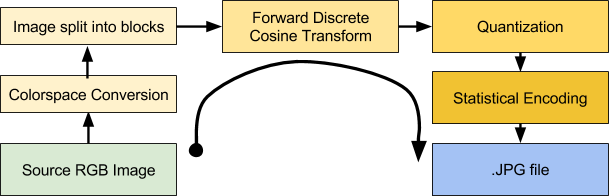
\includegraphics[scale=0.50]{pics/jpegcompression.png}
\caption{Steps involved in JPEG Compression\cite{Jpeg}}
\label{fig:Rec_Acc}
\end{figure}

\begin{figure}[]
\centering
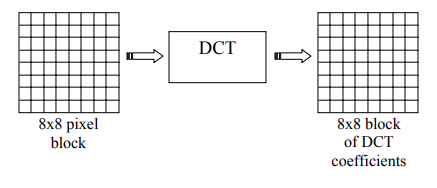
\includegraphics[scale=1]{pics/dct.PNG}
\caption{DCT involved in JPEG\cite{dct}}
\label{fig:Rec_Acc}
\end{figure}
\subsection{Masks and Reconstruction Algorithms}
The main aim of designing a lensless camera is that it would help reduce the size of the camera considerably. In a lensed camera, light emanating from multiple-points in the object would intersect to form the image of the object. This is illustrated in Figure \ref{fig:lens_image}. the focal length of the lens-involed primarily determines the thickness of the camera(See Figure \ref{fig:focal_length}). In a lensless imaging system, the lens is replaced by means of a mask(series of pinholes arranged in a periodic manner). This is illustrated in Figure \ref{fig:lensvslensless}.
\begin{figure}[ht]
\centering
\begin{subfigure}{0.75\textwidth}
  \centering
  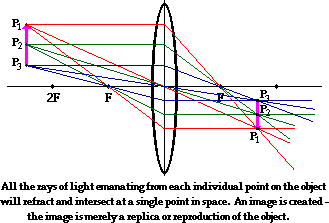
\includegraphics[width=.5\linewidth]{pics/lensed_image_formation}
  \caption{Image Formation in a lens-based camera\cite{lens1}}
  \label{fig:lens_image}
\end{subfigure}
\begin{subfigure}{0.75\textwidth}
  \centering
  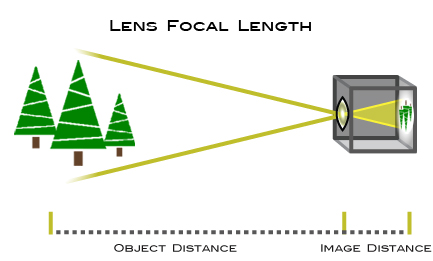
\includegraphics[width=.65\linewidth]{pics/focal_length}
  \caption{Image Distance dictated by focal length \cite{lens2}}
  \label{fig:focal_length}
\end{subfigure}
\caption{Lens-based Camera}
\label{fig:lens_based}
\end{figure}

The simplest lensless imaging system is the pinhole camera. However, since the quality of the image depends on the size of the pinhole, that restricts the amount of light that can enter the imaging system. Lenses were introduced to focus the light from distant objects onto a film or a sensor. In the absence of a lens, the sensor would record the average intensity of the light entering it. This can also bee seen in the experiments which are described in the upcoming chapters. 
\begin{figure}[ht]
\centering
\begin{subfigure}{\textwidth}
  \centering
  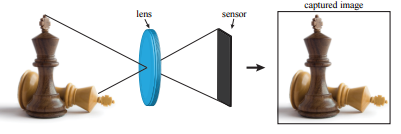
\includegraphics[width=0.75\linewidth]{pics/lensless_1}
  \caption{Conventional Lensed Imaging}
  \label{fig:lensed_imaging}
\end{subfigure}
\begin{subfigure}{\textwidth}
  \centering
  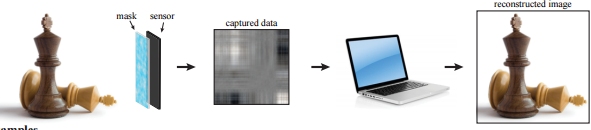
\includegraphics[width=0.75\linewidth]{pics/lensless_2}
  \caption{Lensless Imaging}
  \label{fig:lensless_imaging}
\end{subfigure}
\caption{Difference between lensed and lensless imaging methods\cite{VBoomi}}
\label{fig:lensvslensless}
\end{figure}

In 1960s, Fernimore and Canon introduced Fresnel Zone Plates for a "large aperture, high resolution camera with neither refracting or reflecting components"\cite{Cannon1}. The fresnel zone plate is defined such that the radius of the $n^th$ zone is given by 
\begin{equation}
r_n  = r_1 \sqrt{n}
\end{equation}
An example of Fresnel Zone plate is shown in Figure \ref{fig:fzp}. Fresnel Zone Plates can be used in the places of lenses to produce images because FZPs produce images at multiple higher order foci depending on the type of fresnel plate used. The fresnel zone plates have a transmission of exactly 50 percent. It is always desirable to have an optical system with ideal system point spread function(SPSF). The point spread function describes the response of an optical system to a point source. It can also be called as the impulse response of the optical system. The ideal point spread function of an optical system would be a dirac-delta function. However, in-order to obtain such response with a fresnel zone plate, it would have to be infinite. So, different forms of coded-apertures were developed to overcome the limitations associated with fresnel zone plates. 

\begin{figure}[ht]
\centering
\begin{subfigure}{0.75\textwidth}
  \centering
  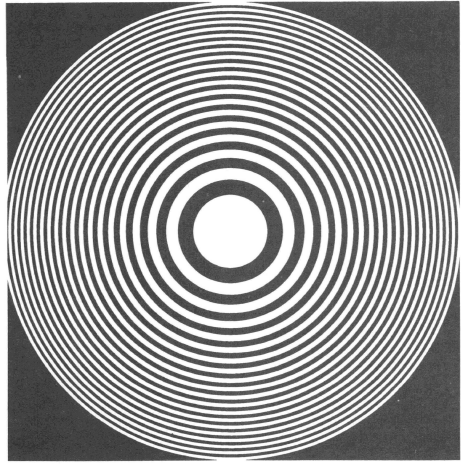
\includegraphics[width=0.50\linewidth]{pics/fzp}
  \caption{A twenty ring Fresnel Zone Plates}
  \label{fig:fzp}
\end{subfigure}
\hfill
\begin{subfigure}{\textwidth}
  \centering
  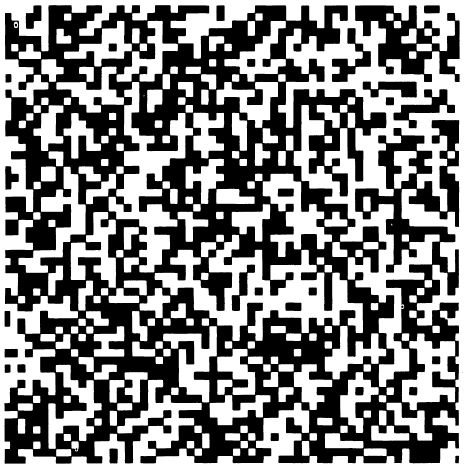
\includegraphics[width=0.50\linewidth]{pics/random_array}
  \caption{A 60*60 Random Array}
  \label{fig:random_array}
\end{subfigure}
\hfill
\begin{subfigure}{\textwidth}
  \centering
  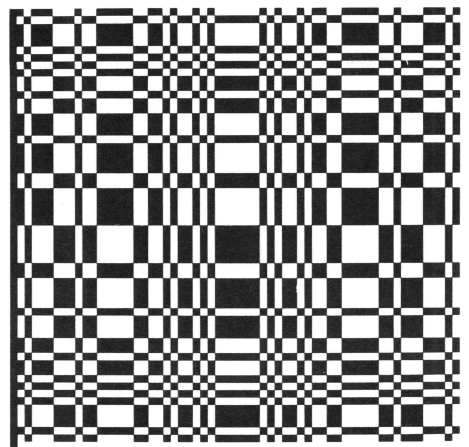
\includegraphics[width=0.50\linewidth]{pics/ura}
  \caption{A 61*59 Uniformly redundant array}
  \label{fig:ura}
\end{subfigure}

\caption{Masks developed initally for lensless imaging\cite{Cannon1}}
\label{fig:lensvslensless}
\end{figure}

Coded aperture cameras extend the pinhole camera concept replacing the single aperture with a mask containing multiple apertures. The first developed coded aperture cameras were used in imaging X-Ray sources due to the difficulty involved in focussing light from X-Ray sources\cite{Cannon1}. Since a single pinhole limits the amount of light imaged by the sensing element, it was replaced by many holes, called the aperture so that overlapping images are formed on the film. The recorded image will have no similarity with the source and an digital processing is required to reconstruct the source image or the object. The recorded image is mathematically modelled as a  collection of overlapping shadows as described by the following equation\cite{VBoomi}\cite{Cannon1} 
\begin{equation}
y = \phi * x + e
\label{eq:conv}
\end{equation}
where $y$ represents the image formed on the sensor, $\phi$ represents the mask pattern, $x$ represents the irradiance vector or the object and $e$ represents the noise. The $*$ operator represents the convolution operation between the mask an the object. The coded aperture increases the flux that falls on the detector and this leads to an increase in the SNR. The SNR can be as large $\sqrt{N}$, where N represents the number of holes in the aperture\cite{Cannon1}. The increased SNR comes at the cost of computational decoding for the image. We can obtain the actual object image $x$ using the inverse of the mask function. An ideal point spread optical function would produce a dirac-delta response $\phi * \phi^-1$.
In 1968, Dicke and Ables\cite{Cannon1} introduced random arrays as am alternative coded aperture imaging method. The mask consists of randomly positioned holes in an opaque surface. An example of a random array is shown in Figure \ref{fig:random_array}. The total open area may or may not be equal to the amount of opaqueness. The image produced by random arrays are decoded digitally using auto-correlation analysis of the encoded images\cite{Cannon1}. Like Fresnel Zone Plates, the random array also exhibits an ideal response when the size of the array is infinite which is practically impossible. A new-class of apertures called uniformly redundant arrays(URAs) were developed over the disadvantages associated with random arrays. The uniformly random arrays exhibit a pattern that follows the equation \ref{eq:ura}\cite{Fenimore:78}. The URA have a dimension of $r$ by $s$ with $r - s = 2$. The quation \ref{eq:ura} takes $I  = mod_ri$ and $J  = mod_rj$($i$ and $j$ represent the array index position in x and y)
\begin{equation}
  A(I,J) =
  \begin{cases}
    0 & \text{if $I = 0$} \\
    1 & \text{if $J = 0$ \& $I\neq 0$} \\
    1 & \text{if $C_r(I)C_s(J) = 1$} \\
    0 & \text{otherwise}\\
  \end{cases}
  \label{eq:ura}
\end{equation}
where
\begin{equation}
  C_r(I) =
  \begin{cases}
    1 & \text{if there exists an integer $x$ such that 
    $1<x<r$ 
	such that $I = mod_rx^2$    
    } \\
    -1 & \text{otherwise} \\
  \end{cases}
  \label{eq:ura}
\end{equation}

The matrix used for deconvolution is given by the equation \ref{eq:decura}. This kind of array produces an ideal point spread function. The point spread function of different masks discussed above is shown in Figure \ref{fig:psf_old_mask}.
\begin{equation}
  G(I,J) =
  \begin{cases}
    1 & \text{if $A(i,j) = 1$} \\
    -1 & \text{if $A(i,j) = 0$} \\
  \end{cases}
  \label{eq:decura}
\end{equation}

\begin{figure}[ht]
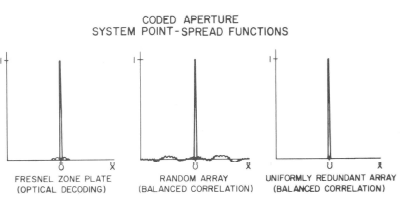
\includegraphics[width=\textwidth]{pics/psf_mask}
\caption{Point Spread function of different masks\cite{Fenimore:78}}
\label{fig:psf_old_mask}
\end{figure}

It can be seen that the Uniformly redundant arrays would offer the best performance and would produce the ideal point spread function. The direct inversion by deconvolution with inverse works when the object is against a dark background with negligible diffraction effects(for example, in the X-Ray Spectrum). 
However, in the later studies\cite{Toeplitz}, it can be seen that equation \ref{eq:conv} no longer holds in the visible light spectrum involving extended-object scenes and direct fourier/deconvolution based reconstruction methods would fail. This is also observed in the simulation studies described in the upcoming chapter. In order to solve the problems associated with reconstructing extended object scenes in the visible light spectrum, a new class of separable Doubly Toeplitz mask was developed by Michael et.al \cite{Toeplitz}. These classes of masks retain their properties even in the presence of diffraction and extended-object scene based scenarios. The doubly toeplitz-masks are expressed as a product of two independent vectors $A(i)$ and $B(j)$.
\begin{equation}
M(i,j) = A(i)B(j)
\end{equation}
If the mask can be expressed in the form of two independent vectors, then the equation \ref{eq:conv} can be re-written in the form: 
\begin{equation}
I = M_AOM_B^T
\label{eq:separable}
\end{equation}

The matrices $M_A$ and $M_B$ are toeplitz meaning they follow the form:

\[ %\arraycolsep=4pt
 M = 
 \begin{bmatrix*}[r]
    A1 & A2 & \cdots &AN & 0 &0 & \cdots & 0 \\
    0 & A1 & A2 & \cdots &AN & 0 & \cdots & 0\\
    \vdots &\cdots &\cdots &\cdots &\cdots&\cdots&\cdots \\
  \end{bmatrix*}
\]

\begin{figure}[ht]

\includegraphics[scale = 0.50]{pics/doubly-topelitz}
\caption{An example of Doubly-Toeplitz Mask\cite{Topelitz}}
\label{fig:doubly_toeplitz}
\end{figure}

Previous studies\cite{Toeplitz}\cite{VBoomi}\cite{Flatcam} have proven that it owuld be possible to perform lensless imaging  in the visible light spectrum for real-life object scenes. The detailed solution and modelling of the computational algorithm would be discussed in the next chapter. This kind of mask would be ideal for our application.